% ============================================================
% CHAPTER 5: RESULTS AND DISCUSSION
% ============================================================

Chapter~4 documented the full implementation of four methods, from preprocessing pipelines and SNOMED RF2 indexing to engineering problems encountered and resolved, and described the deployment tools (annotate\_pdf.py, Streamlit interface) that bridge the benchmark pipeline and real clinical documents. This chapter now evaluates those implementations empirically.

We first report the quantitative evaluation on the MIMIC-IV benchmark across all four methods, analyse the gap between the strict mIoU metric and the ranking quality metrics, examine the qualitative results on six French ophthalmological clinical documents from Cliniques universitaires Saint-Luc including a comparison against two general-purpose AI baselines and an improved M4* variant, report the top-5 hit rate on 36 structured French clinical cases from medical textbooks (Phase~2b), and conclude by revisiting the four working hypotheses formulated in Chapter~1.

\section{Phase 1: Quantitative Results on MIMIC-IV}

\subsection{Full Results Table}

All four methods were evaluated on the 68 test notes for which at least one prediction was produced. The complete quantitative results are presented in Table~\ref{tab:phase1_results}.

\begin{table}[htbp]
\centering
\scriptsize
\caption{Phase~1 quantitative results on MIMIC-IV test split (68 of 72 test notes; 4 notes yielded no predictions across any method). Higher is better. M4 with LLM reranking enabled. Ranking metrics (MRR, NDCG@5, Linear@5, Hits@k) use an IoU $\geq 0.3$ gate; Span Recall and Span F1 use IoU $\geq 0.5$.}
\label{tab:phase1_results}
\adjustbox{max width=\linewidth}{%
\begin{tabular}{lrrrr}
\toprule
\textbf{Metric} & \textbf{M1 (Dict)} & \textbf{M2 (SapBERT)} & \textbf{M3 (LLM+RAG)} & \textbf{M4 (Hybrid)} \\
\midrule
\textbf{mIoU} (primary) & \textbf{0.3601} & 0.1024 & 0.0162 & 0.0398 \\
\midrule
MRR                     & 0.7341 & 0.2598 & 0.4135 & \textbf{0.6796} \\
NDCG@5                  & 0.7426 & 0.2845 & 0.4508 & \textbf{0.6922} \\
Linear@5                & 0.7507 & 0.2982 & 0.4761 & \textbf{0.6994} \\
Hits@1                  & 0.7076 & 0.1990 & 0.3141 & \textbf{0.6484} \\
Hits@3                  & 0.7625 & 0.3197 & 0.5141 & \textbf{0.7101} \\
Hits@5                  & \textbf{0.7671} & 0.3586 & 0.5613 & 0.7298 \\
\midrule
Span Recall             & \textbf{0.4893} & 0.4591 & 0.0449 & 0.0523 \\
Span Precision          & 0.3115 & 0.2771 & \textbf{0.5858} & 0.5830 \\
Span F1                 & 0.3776 & 0.3430 & 0.0819 & \textbf{0.0859} \\
\bottomrule
\end{tabular}}
\end{table}

\begin{figure}[htbp]
\centering
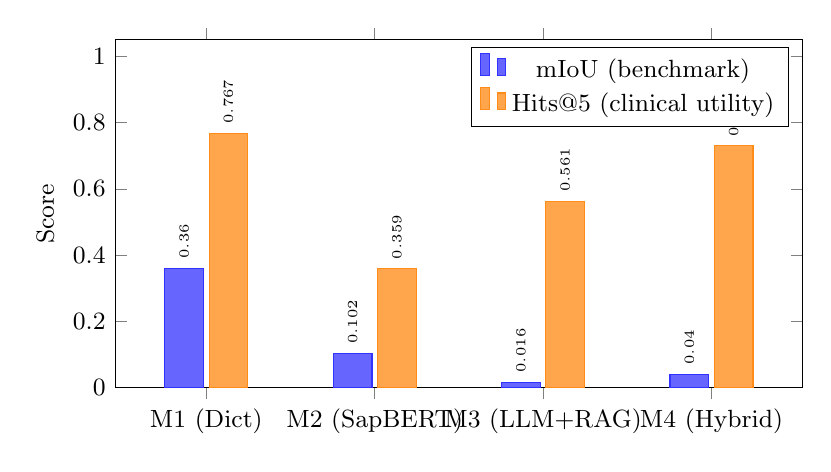
\begin{tikzpicture}
\begin{axis}[
    ybar, bar width=14pt,
    width=0.85\linewidth, height=6cm,
    symbolic x coords={M1 (Dict), M2 (SapBERT), M3 (LLM+RAG), M4 (Hybrid)},
    xtick=data,
    x tick label style={font=\small},
    ymin=0, ymax=1.05,
    ylabel={Score},
    ylabel style={font=\small},
    ytick={0,0.2,0.4,0.6,0.8,1.0},
    yticklabel style={font=\small},
    legend style={at={(0.98,0.98)}, anchor=north east, font=\small},
    enlarge x limits=0.18,
    nodes near coords,
    nodes near coords style={font=\tiny, /pgf/number format/fixed, /pgf/number format/precision=3},
    every node near coord/.append style={rotate=90, anchor=west},
]
\addplot[fill=blue!60, draw=blue!80] coordinates {
    (M1 (Dict),     0.3601)
    (M2 (SapBERT),  0.1024)
    (M3 (LLM+RAG),  0.0162)
    (M4 (Hybrid),   0.0398)
};
\addplot[fill=orange!70, draw=orange!90] coordinates {
    (M1 (Dict),     0.7671)
    (M2 (SapBERT),  0.3586)
    (M3 (LLM+RAG),  0.5613)
    (M4 (Hybrid),   0.7298)
};
\legend{mIoU (benchmark), Hits@5 (clinical utility)}
\end{axis}
\end{tikzpicture}
\caption{mIoU vs.\ Hits@5 for all four methods on the MIMIC-IV test split. The gap between the two bars for Methods~3 and~4 illustrates the annotation density paradox: LLM-based methods achieve high concept linking quality (Hits@5) but are penalised by the exhaustive annotation density of the benchmark (mIoU).}
\label{fig:mimic_results}
\end{figure}

\subsection{Analysis of Method 1}

Method~1 achieves the highest mIoU (0.3601) of all four methods. The mIoU of 0.3601 is competitive with the state of the art on this benchmark: the first-place submission of the SNOMED CT Entity Linking Challenge (KIRI system~\cite{Davidson:2025}) achieved 0.420 mIoU using a dictionary-based approach enriched with UMLS synonyms and section partitioning. Our Method~1 reaches 0.3601 using the training frequency dictionary and SNOMED RF2 synonyms alone, validating the approach. Method~1 also achieves the highest Hits@5 (0.7671) among all four methods.

The MRR of 0.7341 reveals an important structural characteristic of Method~1: \textit{when a span is detected, the concept ranking is very good}. An MRR of 0.7341 indicates strong concept ranking performance; while MRR cannot be directly equated to the proportion of top-1 correct predictions, it is consistent with a high proportion of cases where the correct concept ranks first or second. The Hits@5 of 0.7671 is only marginally higher than the MRR, confirming that Method~1 is calibrated and does not need the full candidate list to find the right answer.

The span recall of 0.4893 is, however, the critical bottleneck. Approximately 51\% of gold annotations in the test set are never covered by any predicted span with IoU $\geq 0.5$. Note that this span recall uses an IoU threshold of $\geq 0.5$; the ranking quality metrics in Table~\ref{tab:phase1_results} (MRR, Hits@k) apply the looser gate of $\geq 0.3$, as specified in Section~3.3.3. These missed spans arise from two sources: clinical expressions that do not appear in either the training dictionary or the SNOMED RF2 synonym list (out-of-vocabulary entities), and expressions whose length exceeds the 8-token sliding window limit. The gap between MRR (0.7341) and mIoU (0.3601) is entirely explained by this span recall deficit: a method that ranks concepts perfectly can still achieve a low mIoU if it fails to detect more than half of the gold spans.

\subsection{Analysis of Method 2}

Method~2 achieves an mIoU of 0.1024, substantially below Method~1. This result is counterintuitive given that SapBERT is a specialised biomedical embedding model that encodes medical synonym relationships. H1 is not confirmed on the English MIMIC-IV benchmark; whether it holds on French ophthalmological text remains partially open, as the qualitative evaluation sample is insufficient for definitive conclusion. Understanding why Method~2 underperforms requires examining the nature of the dataset.

The MIMIC-IV benchmark annotations were largely derived from the SNOMED CT official terminology: annotators identified text spans that match known SNOMED descriptions and assigned the corresponding concept identifiers. This means that the vast majority of annotated spans are, in fact, exact or near-exact matches to SNOMED synonyms already present in the RF2 file. For such in-vocabulary spans, exact string matching (Method~1 Tier~2) achieves a score of 0.95 and retrieves the correct concept with certainty. SapBERT's semantic similarity approach introduces noise: a clinical span such as ``Type 2 diabetes mellitus'' may be semantically closest to ``Type~2 diabetes with complications'' in the embedding space, even though it should map to the canonical code for uncomplicated Type~2 diabetes.

Furthermore, as described in Chapter~4 (Problem~4), the hybrid pre-filtering that makes Method~2 viable already imports the span detection quality of Method~1. The SapBERT component then only adds value for spans where exact matching failed, but for those spans the dictionary score would have been below Tier~2 threshold, and the SapBERT retrieval is operating in a domain where the training annotations provide little supervision. This structural limitation explains why the MRR of Method~2 (0.2598) is substantially below that of Method~1 (0.7341).

The span recall of Method~2 (0.4591) is slightly lower than Method~1 (0.4893) because the hybrid pre-filter is strictly less permissive than Method~1's full lookup chain: a span that would match via Tier~3 fuzzy in Method~1 receives no SapBERT linking in Method~2 (the fuzzy match is not part of the pre-filter). This design decision was intentional (using only exact matches as the pre-filter maintains high precision) but it reduces span coverage.

\subsection{The Annotation Density Paradox: Methods 3 and 4}
\label{sec:annotation_density_paradox}

The mIoU scores of Method~3 (0.0162) and Method~4 (0.0398) are dramatically lower than Methods~1 and~2, despite their MRR values (0.4135 and 0.6796) and Hits@5 values (0.5613 and 0.7298) being competitive. Figure~\ref{fig:mimic_results} makes this contrast immediately visible. This apparent paradox requires careful explanation.

The LLM-based methods instruct the language model to extract \textit{clinically meaningful} medical entities from the note, typically the diagnoses, procedures, and significant findings. In practice, \texttt{llama3.1:8b} extracts approximately 30--40 entities per note, representing the most salient clinical content. The MIMIC-IV gold annotations, by contrast, contain approximately 340 annotations per note, labelling virtually every medical term including highly generic expressions such as ``patient'', ``history of'', ``daily'', and ``oral medication''.

The mIoU metric treats each of the $\sim$340 gold annotations as an independent test case. When a method produces only 40 predictions, it scores 0 on the approximately 300 gold annotations it does not cover. Even if those 40 predictions are perfectly correct (IoU~$=1.0$, correct concept), the resulting mIoU is approximately $40/340 \approx 0.12$, and in practice lower due to imperfect boundaries and concept errors.

This low mIoU score does not indicate a failure of clinical utility; rather, it reflects a fundamental mismatch between the LLM-based methods' selective extraction strategy and the benchmark's exhaustive annotation philosophy. It reflects a \textit{mismatch between evaluation protocol and intended use}. The MIMIC-IV benchmark was designed to evaluate the completeness of automated annotation pipelines: systems are expected to label everything. The LLM-based methods are designed to support a physician in quickly identifying the most important diagnoses from a note, a task for which exhaustive annotation of every medical term is neither desired nor useful.

The Hits@5 of Method~4 (0.7298) compared to its mIoU (0.0398) is the most informative statistic: it states that when Method~4 does identify a span that overlaps a gold annotation, it places the correct SNOMED concept within the top-5 candidates 73.0\% of the time. Method~4's MRR of 0.6796 further confirms that, conditional on finding the span, it places the correct concept at rank~1 approximately 68\% of the time, the highest MRR across all four methods. Method~3's MRR (0.4135) and Hits@5 (0.5613) are also substantially better than Method~2, highlighting that the ranking quality of LLM-based approaches is strong; the mIoU deficit is due solely to the selective extraction mismatch and not to concept linking failures.

\begin{figure}[htbp]
\centering
\begin{tikzpicture}[font=\small]
  % ── shared note background ─────────────────────────────────────────────────
  \def\noteW{5.8} \def\noteH{3.4}

  % LEFT: exhaustive benchmark annotations (~340)
  \node[draw=gray!60, fill=gray!8, rounded corners=3pt,
        minimum width=\noteW cm, minimum height=\noteH cm,
        anchor=north west] (noteL) at (0,0) {};
  \node[above=2pt of noteL.north, font=\bfseries\small] {MIMIC-IV benchmark};
  % dense coloured spans simulating ~340 annotations
  \foreach \x/\w/\col in {
    0.10/1.1/blue!50, 1.30/0.7/green!55, 2.15/0.9/orange!55, 3.20/0.8/red!45,
    4.20/0.6/purple!45, 0.10/0.5/cyan!50, 0.75/0.9/blue!35, 1.80/0.6/green!40,
    2.55/0.5/orange!40, 3.25/0.9/red!35, 4.30/0.4/purple!35,
    0.15/0.8/blue!50, 1.10/1.0/green!50, 2.25/0.7/orange!50, 3.10/0.7/red!45,
    4.00/0.7/cyan!45, 0.20/0.5/purple!40, 0.85/0.8/blue!40, 1.75/0.5/green!35,
    2.40/0.8/orange!35, 3.30/0.6/red!30, 4.10/0.6/blue!30,
    0.10/0.6/cyan!40, 0.85/0.7/purple!30, 1.65/0.9/blue!50, 2.65/0.5/green!45,
    3.25/0.8/orange!45, 4.20/0.5/red!40} {
    \fill[\col, rounded corners=1pt]
      ([xshift=\x cm+0.1cm, yshift=-0.35cm]noteL.north west)
      rectangle +(\w cm, 0.22cm);
    \fill[\col, rounded corners=1pt]
      ([xshift=\x cm+0.1cm, yshift=-0.72cm]noteL.north west)
      rectangle +(\w cm, 0.22cm);
    \fill[\col, rounded corners=1pt]
      ([xshift=\x cm+0.1cm, yshift=-1.09cm]noteL.north west)
      rectangle +(\w cm, 0.22cm);
    \fill[\col, rounded corners=1pt]
      ([xshift=\x cm+0.1cm, yshift=-1.46cm]noteL.north west)
      rectangle +(\w cm, 0.22cm);
  }
  \node[below=6pt of noteL.south, align=center, font=\small]
    {\textbf{\textasciitilde{}340 gold annotations} per note\\
     {\footnotesize Every medical term labelled}};

  % ── dividing arrow ──────────────────────────────────────────────────────────
  \draw[->, thick, gray!70] (6.2,-1.5) -- (7.0,-1.5)
    node[midway, above, font=\scriptsize, align=center] {LLM\\selective\\extraction};

  % RIGHT: LLM-extracted spans (~35)
  \node[draw=gray!60, fill=gray!8, rounded corners=3pt,
        minimum width=\noteW cm, minimum height=\noteH cm,
        anchor=north west] (noteR) at (7.2,0) {};
  \node[above=2pt of noteR.north, font=\bfseries\small] {LLM methods (M3, M4)};
  % sparse clinically meaningful spans
  \foreach \x/\w/\col in {
    0.30/1.8/blue!60,
    2.50/1.4/orange!60,
    0.50/1.2/red!50,
    2.20/1.6/green!55,
    0.40/0.9/purple!50,
    3.20/1.0/cyan!55} {
    \fill[\col, rounded corners=2pt]
      ([xshift=\x cm, yshift=-0.42cm]noteR.north west)
      rectangle +(\w cm, 0.26cm);
    \fill[\col, rounded corners=2pt]
      ([xshift=\x cm, yshift=-1.08cm]noteR.north west)
      rectangle +(\w cm, 0.26cm);
    \fill[\col, rounded corners=2pt]
      ([xshift=\x cm, yshift=-1.74cm]noteR.north west)
      rectangle +(\w cm, 0.26cm);
  }
  \node[below=6pt of noteR.south, align=center, font=\small]
    {\textbf{\textasciitilde{}35 extracted spans} per note\\
     {\footnotesize Clinically significant entities only}};

  % ── Legend ────────────────────────────────────────────────────────────────
  \node[anchor=north west, font=\scriptsize] (leg) at (0,-5.2) {\textbf{SNOMED CT semantic type:}};
  \foreach \col/\lbl/\i in {
      blue!55/Disorder/0,
      green!55/Finding/1,
      orange!55/Procedure/2,
      red!50/Body structure/3,
      purple!50/Substance/4,
      cyan!55/Observable entity/5} {
    \fill[\col, rounded corners=1pt]
      ([xshift=\i*2.15cm, yshift=-0.35cm]leg.south west)
      rectangle ++(0.45cm, 0.22cm);
    \node[anchor=west, font=\scriptsize]
      at ([xshift=\i*2.15cm+0.52cm, yshift=-0.24cm]leg.south west) {\lbl};
  }

\end{tikzpicture}
\caption{The annotation density paradox. The MIMIC-IV benchmark labels every medical term exhaustively ($\sim$340 annotations per note). LLM-based methods extract only clinically meaningful entities ($\sim$35 per note). The mIoU metric scores zero on every unmatched gold annotation, penalising selective methods regardless of their concept linking quality.}
\label{fig:annotation_density}
\end{figure}

\section{Phase 2: Qualitative Evaluation on French Clinical PDFs}

\subsection{Evaluation Setup}

Six anonymised ophthalmological PDF documents from Cliniques universitaires Saint-Luc were annotated by all four methods. The ground truth is the problem list encoded by the treating physician in the Epic EHR system. This evaluation is qualitative in nature: the small sample size (16 evaluable diagnoses across 5 documents; one document has an empty Epic problem list) does not support statistical inference. The reason for the empty Epic problem list for PDF~3 could not be determined from available information; possibilities include coding omission, absence of active problems at the time of visit, or preliminary note status. This uncertainty is acknowledged as a limitation of the qualitative evaluation. It nonetheless provides the only currently available signal about method performance on the actual target language and domain.

In addition to the four automated methods, two general-purpose large language models were evaluated directly: GPT-3.5 and Claude Sonnet~4.6. Both models received the raw French PDF text and were prompted to identify diagnoses with matching SNOMED CT concept codes using the following structured prompt:

\begin{quote}
\textit{Analyze the attached medical PDF. Extract all clinical problems/findings mentioned in the ``Note'' section. For each problem found, output a line in this exact format: PROBLEM | SNOMED CODE | SNOMED LABEL. Rules: only include clinically significant problems/findings (diagnoses, active conditions, relevant findings); use the most specific SNOMED CT code available; if no confident SNOMED code exists, write UNKNOWN; no explanations, no headers, no extra text; one line per problem.}
\end{quote}

Unlike Methods~3 and~4, these AI baselines have no access to the SNOMED FAISS index or training dictionary: concept codes were generated from the model's knowledge without retrieval grounding. The prompt instructs both models to include all clinically significant problems without restricting to ophthalmic findings, which as discussed below proves advantageous for capturing systemic comorbidities. A diagnosis is counted as found if the model identifies it with a correct or semantically equivalent SNOMED concept identifier.

An additional variant, M4*, was also evaluated: it applies the same two improvements to Method~4 that were motivated by the AI baseline analysis: an expanded NER scope instruction covering systemic comorbidities, and a chunking mechanism replacing the previous 8\,000-character hard truncation of long notes.

Table~\ref{tab:french_qualitative} presents the results for all seven systems.

\begin{table}[htbp]
\centering
\scriptsize
\caption{Qualitative evaluation on 6 French PDFs from Saint-Luc (PDF~3 excluded: Epic list empty). \textbf{Illustrative only: n\,=\,16 diagnoses; no statistical inference is warranted.} Gold: Epic problem list. M1--M4 use top-10 candidate threshold; M4* is M4 with improved NER prompt (comorbidities scope) and note chunking; GPT-3.5 and Claude use parametric SNOMED knowledge.}
\label{tab:french_qualitative}
\adjustbox{max width=\linewidth}{%
\begin{tabular}{L{0.9cm}L{1.8cm}L{3.4cm}ccccccc}
\toprule
\textbf{PDF} & \textbf{Specialty} & \textbf{Epic diagnoses} & \textbf{M1} & \textbf{M2} & \textbf{M3} & \textbf{M4} & \textbf{M4*} & \textbf{GPT-3.5} & \textbf{Claude S.} \\
\midrule
PDF~1 & Retina & panuvéite virale; HTA; RGO & 0/3 & 0/3 & 0/3 & 0/3 & 0/3 & 0/3 & 0/3 \\
PDF~2 & Strabismus & exotropie intermittente & 1/1 & 1/1 & 1/1 & 1/1 & 1/1 & 1/1 & 1/1 \\
PDF~3 & Oncology & \textit{(Epic list empty)} & \multicolumn{7}{c}{\textit{Non-evaluable}} \\
PDF~4 & Neuro-ophth. & paralysie VI; HTA; épiphora; cataracte OD; HTO & 3/5 & 2/5 & 3/5 & 3/5 & \textbf{5/5} & \textbf{5/5} & \textbf{5/5} \\
PDF~5 & Cornea & dystrophie endothéliale de Fuchs & 0/1 & 0/1 & 1/1 & 1/1 & 1/1 & 1/1 & 1/1 \\
PDF~6 & Neuro-ophth. & HTA; fibrill. atriale; hypothyroïdie; cataracte (×2); strabisme & 2/6 & 2/6 & 2/6 & 2/6 & 2/6 & 1/6 & 1/6 \\
\midrule
\textbf{Total} & & \textbf{16 diagnoses} & 37.5\% & 31.3\% & 43.8\% & 43.8\% & \textbf{56.3\%} & 50.0\% & 50.0\% \\
\bottomrule
\end{tabular}}
\end{table}

\subsection{AI Baseline Comparison}

GPT-3.5 was selected as a cost-effective and widely accessible baseline representative of non-proprietary-scale language models. A comparison against GPT-4o or equivalent current-generation models is identified as a direction for future work.

Both GPT-3.5 and Claude Sonnet~4.6 achieve \textbf{50.0\%} (8/16 diagnoses), outperforming the four original automated methods but falling short of M4* (56.3\%).

The prompt improvement in M4*, adding an explicit scope instruction for systemic comorbidities and a note-chunking mechanism to prevent content loss on long documents, raises M4 from 43.8\% to 56.3\%, surpassing both AI baselines (50.0\%). The gain is concentrated entirely on PDF~4, where the updated NER prompt now instructs the LLM to include conditions such as hypertension that appear in the background history rather than the main ophthalmological findings. M4* recovers all five Epic diagnoses for PDF~4 (5/5) compared to only three before the fix.

PDF~6 scores remain identical between M4 and M4* (2/6): the updated method correctly identifies strabisme and cataracte OD, while fibrill. atriale is detected as ``embolisation sur une FA'' (mapped to Embolism rather than Atrial fibrillation) and hypothyroïdie remains absent from the extracted note text. The AI baselines score only 1/6 on PDF~6, missing strabisme entirely.

PDF~1 remains unsolvable for all methods (0/3): the treating diagnosis of viral panuveitis is clinically implied by the described retinal findings but never stated explicitly in the note.

It is important to note a fundamental methodological difference: M4* relies on a curated SNOMED RF2 index and a FAISS vector search over 529k concepts to ground its outputs. The AI baselines generate SNOMED concept codes from parametric knowledge alone, which introduces a risk of hallucinated or outdated concept identifiers. In this evaluation, both AI models produced valid SNOMED codes for every diagnosis they identified; however, this cannot be guaranteed at scale, and the automated methods offer stronger guarantees of concept validity.

\subsection{Key Observations}

Several patterns emerge from the qualitative evaluation.

\textbf{Methods~3 and~4 outperform Methods~1 and~2 on French text.} The order of methods is reversed relative to the English MIMIC-IV benchmark: M3 and M4 (43.8\%) outperform M1 (37.5\%) and M2 (31.3\%). This reversal is attributable to the LLM's native French language comprehension. The \texttt{llama3.1:8b} model reads French clinical prose directly and identifies the most salient diagnoses without requiring the exhaustive annotation coverage demanded by MIMIC-IV. In a sparse-label evaluation like the Epic problem list, the LLM's selective extraction is an asset rather than a liability.

\textbf{The decisive diagnostic in PDF~5 is identified by all LLM-based methods but not by Methods~1 and~2.} ``Dystrophie endothéliale de Fuchs'' was correctly retrieved by Methods~3, M4, M4*, GPT-3.5, and Claude Sonnet~4.6, but missed by Methods~1 and~2. The term appeared in the clinical note as ``dystrophie de Fuchs'' (an abbreviated form) rather than the full official SNOMED synonym. All LLM-based approaches understood from context that this referred to Fuchs endothelial dystrophy; Method~1's dictionary failed because the exact normalised key was not present in either the training frequency dictionary or the RF2 synonyms under that abbreviated form.

\textbf{No method recovers the diagnoses of PDF~1} (viral panuveitis, hypertension, gastro-oesophageal reflux). The retina note describes the retinal manifestations of panuveitis in detail without ever using the word ``panuvéite'' explicitly: the diagnosis is implicit in the clinical description. This is a fundamental limitation of all four methods: they can link expressed terms to SNOMED concepts but cannot infer diagnoses that are clinically implied but not verbally stated.

\textbf{Systemic conditions in PDF~6 are undetectable.} The Epic problem list for PDF~6 includes atrial fibrillation and hypothyroidism, systemic conditions managed by another specialty that appear in the ophthalmological note only as co-morbidities mentioned in the patient history but not described in clinical detail. No method can be expected to detect these from an ophthalmological consultation note, and their absence from the results is expected.

\textbf{Methods~3 and~4 achieve identical scores on the French PDFs (43.8\%)}, suggesting that the gain from Method~4's tiered dictionary over Method~3's pure FAISS approach is not observable on this small sample. The advantage of exact dictionary matching is most visible when the corpus contains many repeated standard terminology items, a condition better satisfied by a larger annotated corpus than by 16 diagnoses across 5 documents. However, M4* demonstrates that targeted improvements to the LLM NER component, rather than to the concept linking stage, yield the largest gains on French clinical text, raising performance to 56.3\%.

\section{Phase 2b: Evaluation on Structured French Clinical Cases}

To complement the small-sample PDF evaluation with a larger French-language signal, a second evaluation was conducted on 36 structured clinical cases drawn from French medical textbooks: 1 English ophthalmology case~\cite{Friedman:2022}, 12 French ophthalmology cases~\cite{COUF:2013}, and 23 French cardiology cases~\cite{CNEC:2015}. A total of 270 gold concept annotations were created, initially generated by a large language model then verified against the SNOMED CT International Release (March 2026): 31 retired identifiers were replaced with their active equivalents, 5 semantically incorrect identifiers were manually corrected, and 26 French-language labels were realigned to the concept identifiers returned by the Belgian RF2 French synonym dictionary to remove evaluation artefacts caused by SNOMED's multiple near-equivalent concepts for the same clinical notion. Additionally, three targeted improvements were applied to Method~4 prior to this evaluation: (1)~French ligature normalisation (œ\,$\rightarrow$\,oe) in the dictionary key hash function; (2)~abbreviation expansion applied before Tier~1/2 lookup as well as before FAISS; and (3)~progressive prefix trimming, which retries progressively shorter token prefixes when a full extracted span misses the dictionary, recovering cases such as ``dyspnée d'effort ancienne'' $\rightarrow$ ``dyspnée d'effort''. Table~\ref{tab:cas_cliniques_results} reports the top-5 hit rate by section; a hit is counted when the correct SNOMED concept identifier appears in the top-5 candidates of any predicted span within the case.

\begin{table}[htbp]
\centering
\scriptsize
\caption{Top-5 hit rate on \texttt{cas\_cliniques} (36 cases, 270 gold annotations). M1--M4: top-5 candidates across all spans; Claude~S. and GPT-3.5: exact SNOMED concept match (same prompt, no retrieval index). M4 and M4$_{\text{rerank}}$ score identically on top-5 hit rate: reranking reorders candidates within the top-5 (improving Hits@1 and MRR) but does not change top-5 presence.}
\label{tab:cas_cliniques_results}
\adjustbox{max width=\linewidth}{%
\begin{tabular}{lrrrrrrr}
\toprule
\textbf{Section} & \textbf{Gold} & \textbf{M1} & \textbf{M2} & \textbf{M3} & \textbf{M4 / M4$_{\text{rerank}}$} & \textbf{Claude~S.} & \textbf{GPT-3.5} \\
\midrule
Ophthalmology (EN) &   5 & 80\% & 60\% & 80\% & 80\% & 20\% & 40\% \\
Ophthalmology (FR) &  82 & 20\% & 13\% & 32\% & 38\% & 38\% & 24\% \\
Cardiology (FR)    & 183 & 33\% & 22\% & 27\% & 42\% & 31\% & 30\% \\
\midrule
\textbf{Overall}   & \textbf{270} & \textbf{30\%} & \textbf{20\%} & \textbf{29\%} & \textbf{42\%} & \textbf{33\%} & \textbf{29\%} \\
\bottomrule
\end{tabular}}
\end{table}

\textbf{Method~4 leads on all French sections} (Figure~\ref{fig:french_results}). Without reranking, M4 achieves the highest overall score~(42\%), outperforming M3~(29\%), M1~(30\%), and M2~(20\%). The gain is largest in cardiology~(42\% vs 27\% for M3), where the progressive prefix-trimming improvement recovers French clinical spans with qualifying modifiers that exact-match lookup would otherwise miss (\eg ``dyspnée d'effort ancienne'' trimmed to ``dyspnée d'effort'').

\textbf{Claude~Sonnet~4.6 matches M4 on French ophthalmology.} Claude achieves 38\% on the French ophthalmology section, tied with M4, without access to any retrieval index: concept codes are generated from parametric knowledge alone. This confirms the pattern observed on the Saint-Luc PDFs: frontier LLMs have competitive recall on ophthalmological French text, but the advantage does not extend to cardiology~(31\%), where M4's tiered dictionary with French synonyms provides a structural edge.

\textbf{GPT-3.5 and M3 perform comparably overall~(29\%)} but with different error profiles: GPT-3.5 scores higher on the English case~(40\% vs 29\% for M3) but lower on French ophthalmology~(24\% vs 32\%), suggesting stronger English parametric coverage but weaker French ophthalmological vocabulary compared to the LLM-plus-RAG approach.

\textbf{Method~2 underperforms systematically.} SapBERT achieves only 13\% on French ophthalmology and 22\% on French cardiology, the lowest scores across all methods on the French sections. The English-only SapBERT embedding space does not reliably align French clinical queries with the English SNOMED concept space; the multilingual SapBERT variant (\texttt{cambridgeltl/SapBERT-UMLS-2020AB-all-lang-from-XLMR}) is the appropriate replacement for French deployment.

\textbf{AI baselines lack SNOMED grounding guarantees.} Claude and GPT-3.5 generate concept identifiers from parametric knowledge; any code not present in the active SNOMED CT release is silently wrong. In this evaluation, most codes produced were valid, but this cannot be guaranteed at scale. M1--M4 retrieve concepts exclusively from the verified RF2 index, providing stronger guarantees of concept validity for clinical deployment.

\subsection{Combined French Evaluation Summary}

Taken together, the two French evaluation corpora (6 Saint-Luc PDFs, 16 diagnoses; 36 textbook clinical cases, 270 annotations) provide converging evidence for the same ranking reversal observed relative to the MIMIC-IV benchmark. Table~\ref{tab:french_combined} summarises Method~4's position across all three evaluation contexts.

\begin{table}[htbp]
\centering
\scriptsize
\caption{Method~4 top-5 hit rate across all evaluation contexts.}
\label{tab:french_combined}
\adjustbox{max width=\linewidth}{%
\begin{tabular}{L{4cm}rL{2cm}L{5.5cm}}
\toprule
\textbf{Corpus} & \textbf{Cases} & \textbf{M4} & \textbf{Note} \\
\midrule
MIMIC-IV (EN, benchmark) & 68 notes & mIoU 0.040 Hits@5 73\% & Dense annotation; architectural penalty on LLM methods \\
Saint-Luc PDFs (FR) & 5 docs & M4 44\% / M4* 56\% & Real clinical notes; sparse gold standard \\
Textbook cases (FR/EN) & 36 cases & 42\% & Systematic; 270 verified annotations \\
\bottomrule
\end{tabular}}
\end{table}

The convergence across two independent French corpora (totalling 286 gold annotations) strengthens the central finding: LLM-based hybrid methods are better suited to the target clinical setting than the benchmark metric alone would suggest. The Saint-Luc PDFs demonstrate real-world applicability on genuine consultation notes; the textbook cases provide the larger, more systematic signal needed to confirm the pattern across specialties and case types.

\begin{figure}[htbp]
\centering
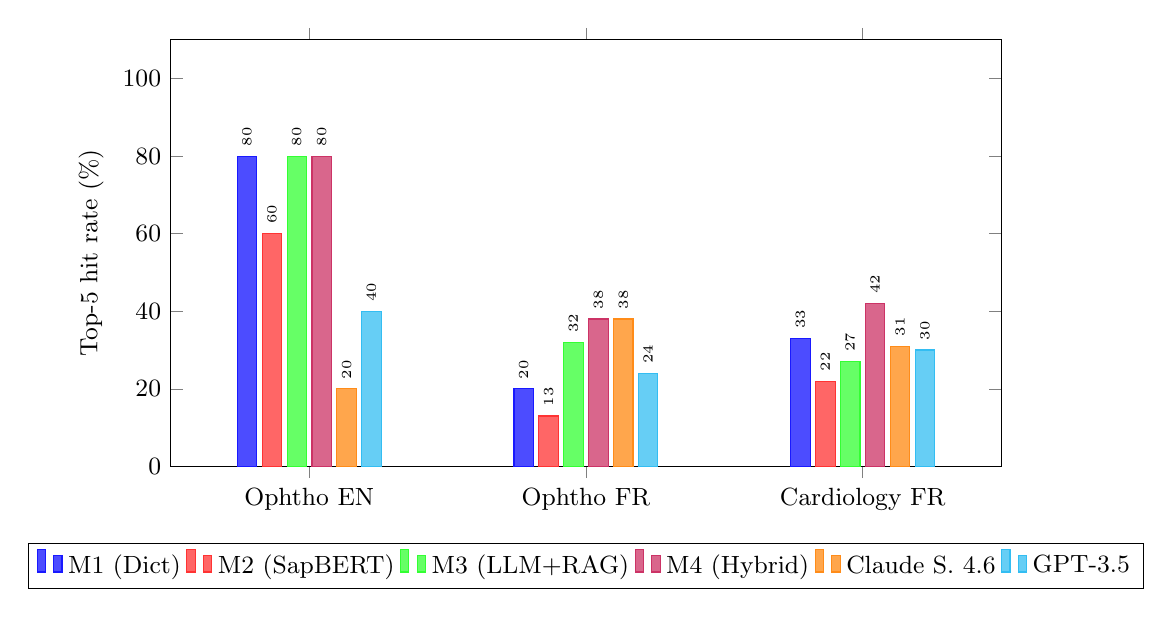
\begin{tikzpicture}
\begin{axis}[
    ybar, bar width=7pt,
    width=\linewidth, height=7cm,
    symbolic x coords={Ophtho EN, Ophtho FR, Cardiology FR},
    xtick=data,
    x tick label style={font=\small},
    ymin=0, ymax=110,
    ylabel={Top-5 hit rate (\%)},
    ylabel style={font=\small},
    ytick={0,20,40,60,80,100},
    yticklabel style={font=\small},
    legend style={at={(0.5,-0.18)}, anchor=north, legend columns=6, font=\small},
    enlarge x limits=0.25,
    nodes near coords,
    nodes near coords style={font=\tiny, rotate=90, anchor=west},
]
\addplot[fill=blue!70,   draw=blue!90]   coordinates {(Ophtho EN,80) (Ophtho FR,20) (Cardiology FR,33)};
\addplot[fill=red!60,    draw=red!80]    coordinates {(Ophtho EN,60) (Ophtho FR,13) (Cardiology FR,22)};
\addplot[fill=green!60,  draw=green!80]  coordinates {(Ophtho EN,80) (Ophtho FR,32) (Cardiology FR,27)};
\addplot[fill=purple!60, draw=purple!80] coordinates {(Ophtho EN,80) (Ophtho FR,38) (Cardiology FR,42)};
\addplot[fill=orange!70, draw=orange!90] coordinates {(Ophtho EN,20) (Ophtho FR,38) (Cardiology FR,31)};
\addplot[fill=cyan!60,   draw=cyan!80]   coordinates {(Ophtho EN,40) (Ophtho FR,24) (Cardiology FR,30)};
\legend{M1 (Dict), M2 (SapBERT), M3 (LLM+RAG), M4 (Hybrid), Claude S.~4.6, GPT-3.5}
\end{axis}
\end{tikzpicture}
\caption{Top-5 hit rate by section on \texttt{cas\_cliniques} (270 gold annotations). M4 leads on both French sections. Claude~Sonnet~4.6 matches M4 on French ophthalmology but falls behind in cardiology, where M4's tiered dictionary with French synonyms provides a structural advantage.}
\label{fig:french_results}
\end{figure}

\section{Comparative Analysis}

\subsection{The Span Recall Bottleneck}

Across all methods, span recall is the primary performance limiter. Table~\ref{tab:span_recall} summarises the span recall values and their relationship to mIoU.

\begin{table}[htbp]
\centering
\scriptsize
\caption{Span recall (IoU $\geq 0.5$) versus mIoU for all four methods.}
\label{tab:span_recall}
\adjustbox{max width=\linewidth}{%
\begin{tabular}{lrrL{5.5cm}}
\toprule
\textbf{Method} & \textbf{Span Recall} & \textbf{mIoU} & \textbf{Primary bottleneck} \\
\midrule
M1 (Dict+Fuzzy) & 0.4893 & 0.3601 & Vocabulary coverage \\
M2 (SapBERT)    & 0.4591 & 0.1024 & Concept linking quality \\
M3 (LLM+RAG)    & 0.0449 & 0.0162 & Selective extraction vs.\ dense annotations \\
M4 (Hybrid)     & 0.0523 & 0.0398 & Selective extraction vs.\ dense annotations \\
\bottomrule
\end{tabular}}
\end{table}

For Methods~1 and~2, the bottleneck is traditional in the sense that more training data and a richer vocabulary would likely close the gap. For Methods~3 and~4, the bottleneck is architectural: improving concept linking quality (as evidenced by the high Hits@5) does not improve mIoU because the fundamental issue is the mismatch between LLM selectivity and benchmark annotation density.

\subsection{The MRR–mIoU Gap}

The gap between MRR and mIoU across all methods can be interpreted as a measure of span detection quality. For Method~1, MRR~(0.7341) is close to Hits@5~(0.7671) and both are substantially above mIoU~(0.3601). The difference is almost entirely explained by the fact that approximately 51\% of gold annotations receive no overlapping prediction. If span recall were perfect (hypothetically 1.0), and the MRR on currently gated annotations (0.7341) were maintained, the resulting mIoU would be approximately $1.0 \times 0.7341 \approx 0.73$, more than double the observed value, under the optimistic assumption that concept linking quality on currently missed spans would match that on detected spans; in practice, currently missed spans are likely harder cases with lower expected MRR. This calculation nonetheless confirms that improving span recall to 0.7--0.8 would be worth approximately as much as perfect concept linking.

\section{Assessment of Working Hypotheses}

Chapter~1 formulated four working hypotheses. We now assess each against the experimental evidence.

\subsection*{H1: Deep learning and BERT-based approaches will outperform dictionary-based methods}

\textbf{Status: Refuted for Phase~1 English benchmark.}

Method~2 (SapBERT, mIoU~0.1024) is substantially outperformed by Method~1 (dictionary, mIoU~0.3601) on the MIMIC-IV benchmark. The hypothesis assumed that semantic representations would capture synonyms and paraphrases better than string matching. This is true in principle but irrelevant in practice for MIMIC-IV: the benchmark annotations are overwhelmingly derived from SNOMED official synonyms, making exact string matching nearly optimal for this corpus. The semantic advantage of SapBERT would be expected to manifest more strongly on a corpus with higher linguistic variability, paraphrasing, and colloquial medical language, characteristics more typical of the French ophthalmological notes at Saint-Luc.

\subsection*{H2: Hybrid approaches combining rules with machine learning will offer the best balance of performance and interpretability}

\textbf{Status: Partially confirmed, but in an unexpected configuration.}

The hypothesis was interpreted as predicting that a fixed rule-machine-learning combination (such as Method~2's dictionary pre-filter with SapBERT concept linking) would be optimal. The results instead reveal that the most effective hybrid is a combination across the \textit{span detection} and \textit{concept linking} stages independently: LLM NER (contextual, data-driven) combined with dictionary lookup (rule-based, deterministic) as in Method~4. Method~4 achieves the highest MRR (0.6796) among all methods on the MIMIC-IV benchmark, confirming that hybrid integration at the pipeline architecture level, rather than within a single module, is the most fruitful design pattern. The qualitative evaluation on French PDFs further reinforces this: M4*, which improves only the LLM NER prompt scope (a targeted intervention in the span detection stage), raises performance from 43.8\% to 56.3\%, surpassing both the original automated methods and the AI baselines (50.0\%).

\subsection*{H3: The scope of the entity extraction prompt significantly affects the detection of comorbidities in LLM-based methods}

\textbf{Status: Confirmed.}

The comparison between Method~4 and M4* directly tests this hypothesis. The original Method~4 prompt instructed \texttt{llama3.1:8b} to extract medical entities that could be mapped to SNOMED CT concepts, without specifying that systemic comorbidities should be included. On PDF~4 (neuro-ophthalmology), this produced only 3/5 Epic diagnoses, missing hypertension (HTA) and ocular hypertension (HTO) which appear in the background history section of the note rather than the main ophthalmic findings.

Adding a single explicit scope instruction: \textit{``Include ALL diagnoses and findings, both primary ophthalmic findings AND systemic comorbidities mentioned anywhere in the note (patient history, background conditions)''} raised PDF~4 from 3/5 to 5/5, and overall French PDF performance from 43.8\% to 56.3\%, confirming the hypothesis. The effect is concentrated on comorbidities embedded in patient history sections, which the model deprioritises without explicit guidance. This finding has direct practical implications for clinical deployment: modifying the entity extraction prompt requires no retraining, no additional computational resources, and no changes to the underlying model, yet it produced a 12.5 percentage point improvement in comorbidity recall (from 43.8\% to 56.3\%) on the French qualitative evaluation.

\subsection*{H4: Adaptation from English to French requires more than direct translation of training data}

\textbf{Status: Supported by preliminary evidence.}

The qualitative evaluation on French PDFs provides initial support: the methods that perform best on French text are those that leverage native French comprehension (LLM-based Methods~3 and~4) rather than those that rely on English-trained string matching (Method~1) or English-centric embeddings (Method~2). Method~1 achieves 37.5\% on French PDFs despite its SNOMED RF2 French extension, suggesting that the French synonym coverage alone is insufficient. The LLM's ability to interpret French clinical syntax and domain-specific abbreviations (``OD'', ``PIO'', ``AV'') proves decisive for this domain.

The combined French evaluation (Section~5.2, 16 diagnoses; Section~5.3, 270 annotations) provides converging evidence: M4 and M3 consistently outperform M1 and M2 across both corpora, confirming that French comprehension requires more than dictionary coverage of RF2 synonyms.

\section{Threats to Validity and Limitations}

\subsection{External Validity}

The primary quantitative evaluation uses a single English dataset (MIMIC-IV discharge summaries), which differs significantly from the target domain (French ophthalmological consultation notes). Discharge summaries are longer, more structured, and written in a more formal register than ophthalmological consultation notes. Performance on MIMIC-IV may not generalise to French ophthalmological text, as suggested by the reversal of method rankings between the two evaluation contexts.

\subsection{Benchmark Annotation Density}

The MIMIC-IV benchmark's exhaustive annotation policy (340 annotations per note) creates an evaluation environment that systematically disadvantages selective methods. mIoU as computed on this benchmark is not a pure measure of concept linking quality; it is partly a measure of whether a method's extraction strategy matches the annotation philosophy. Future work should evaluate all four methods on a French corpus annotated under a clinical-relevance criterion (annotating only primary diagnoses and key findings), which would provide a fairer comparison of concept linking quality.

\subsection{Qualitative Evaluation Sample Size}

The French PDF evaluation involves only six documents and 16 evaluable diagnoses. Statistical conclusions cannot be drawn from this sample. The percentages reported (31.3\% to 56.3\% across all variants) should be interpreted as directional signals rather than precise performance estimates.

\subsection{LLM Non-determinism}

The LLM-based Methods~3 and~4 use \texttt{llama3.1:8b} at temperature~0 (greedy decoding) to maximise reproducibility. Despite this, minor variations in prompt formatting and model loading can produce slightly different outputs across runs. The reported results represent a single evaluation run and have not been averaged over multiple seeds. For the qualitative evaluation in particular (n\,=\,16 diagnoses), a single different LLM decision would shift the reported percentage by 6.25 points. Future work should report results averaged over multiple runs to quantify variance.

\subsection{Method~4 Reranking}

The results reported for Method~4 include the optional LLM reranking step, which performs one additional \texttt{llama3.1:8b} call per batch of 8 candidate spans to re-score the FAISS-retrieved concepts. Reranking raises MRR to 0.6796 and Hits@1 to 0.6484 at the cost of increased inference time relative to a FAISS-only configuration. Evaluating Method~4 without reranking is identified as a direction for future work to quantify the contribution of the reranking component in isolation.
